\documentclass[11pt,a4paper]{article}
\usepackage[margin=0.75in]{geometry}
\usepackage{amsmath,amssymb,mathtools}
\usepackage{array,booktabs,longtable}
\usepackage{enumitem}
\usepackage{tikz}
\usetikzlibrary{arrows.meta,calc,positioning,patterns}
\usepackage{pgfplots}
\pgfplotsset{compat=1.18}
\usepackage{xcolor}
\usepackage{tcolorbox}
\tcbuselibrary{breakable,skins}
\usepackage{fancyhdr}
\usepackage{hyperref}
\hypersetup{colorlinks=true,linkcolor=blue,urlcolor=blue}
\usepackage{microtype}

\definecolor{titleblue}{HTML}{12355B}
\definecolor{lightblue}{HTML}{EAF3FF}
\definecolor{lightgray}{HTML}{F7F7F7}
\definecolor{answergreen}{HTML}{0B6E4F}
\definecolor{warnred}{HTML}{B00020}

\pagestyle{fancy}
\fancyhf{}
\lhead{IGNOU BCS-012: Basic Mathematics}
\rhead{June 2025 Solved Paper}
\cfoot{\thepage}
\setlength{\headheight}{14pt}
\setlength{\parindent}{0pt}
\setlength{\parskip}{5pt}

\newtcolorbox{questionbox}{breakable,enhanced,colback=lightblue,colframe=titleblue,boxrule=0.7pt,arc=2mm,left=1.5mm,right=1.5mm,top=1mm,bottom=1mm}
\newtcolorbox{answerbox}{breakable,enhanced,colback=white,colframe=answergreen,boxrule=0.6pt,arc=2mm,left=1.5mm,right=1.5mm,top=1mm,bottom=1mm}
\newcommand{\question}[1]{\begin{questionbox}\textbf{Question.} #1\end{questionbox}}
\newcommand{\answer}{\begin{answerbox}\textbf{Solution.} }
\newcommand{\eanswer}{\end{answerbox}}
\newcommand{\finalans}[1]{\[\boxed{#1}\]}

\begin{document}

\begin{titlepage}
\centering
\vspace*{1.5cm}
{\Large \textbf{Bachelor of Computer Applications (BCS/BCA)}}\\[0.4cm]
{\Huge \textbf{BCS-012: Basic Mathematics}}\\[0.4cm]
{\LARGE \textbf{Term-End Examination: June 2025}}\\[1cm]
\begin{tcolorbox}[colback=lightgray,colframe=titleblue,width=0.88\textwidth,arc=2mm]
\centering
\textbf{Full Solved Question Paper in LaTeX}\\
Step-by-step solutions, required diagrams/graphs, and final theory/formula sheet.
\end{tcolorbox}
\vfill
\textbf{Time:} 3 Hours \qquad \textbf{Maximum Marks:} 100\\[0.4cm]
\textbf{Note:} Question No. 1 is compulsory. Attempt any three questions from the remaining questions.\\[1cm]
\vfill
{Prepared for exam revision and practice.}
\end{titlepage}

\tableofcontents
\newpage

\section*{Question 1}
\addcontentsline{toc}{section}{Question 1}

\question{(a) Show that
\[
\begin{vmatrix}
b+c&c+a&a+b\\
c+a&a+b&b+c\\
a+b&b+c&c+a
\end{vmatrix}
=2\begin{vmatrix}
a&b&c\\ b&c&a\\ c&a&b
\end{vmatrix}.
\]}
\answer
Let
\[
D_1=\begin{vmatrix}
b+c&c+a&a+b\\
c+a&a+b&b+c\\
a+b&b+c&c+a
\end{vmatrix},\qquad
D_2=\begin{vmatrix}
a&b&c\\ b&c&a\\ c&a&b
\end{vmatrix}.
\]
Both are circulant-type determinants. Expanding the first determinant gives
\[
D_1=-2(a+b+c)(a^2+b^2+c^2-ab-bc-ca).
\]
Similarly,
\[
D_2=-(a+b+c)(a^2+b^2+c^2-ab-bc-ca).
\]
Therefore,
\[
D_1=2D_2.
\]
Hence proved.
\eanswer

\question{(b) If
\[
A=\begin{bmatrix}2&0&1\\2&1&3\\1&-1&0\end{bmatrix},
\]
find \(f(A)\), where \(f(x)=x^2-5x+6\).}
\answer
Here
\[
f(A)=A^2-5A+6I_3.
\]
First,
\[
A^2=\begin{bmatrix}2&0&1\\2&1&3\\1&-1&0\end{bmatrix}
\begin{bmatrix}2&0&1\\2&1&3\\1&-1&0\end{bmatrix}
=\begin{bmatrix}5&-1&2\\9&-2&5\\0&-1&-2\end{bmatrix}.
\]
Also,
\[
-5A=\begin{bmatrix}-10&0&-5\\-10&-5&-15\\-5&5&0\end{bmatrix},\qquad
6I_3=\begin{bmatrix}6&0&0\\0&6&0\\0&0&6\end{bmatrix}.
\]
Thus
\[
f(A)=\begin{bmatrix}5&-1&2\\9&-2&5\\0&-1&-2\end{bmatrix}
+\begin{bmatrix}-10&0&-5\\-10&-5&-15\\-5&5&0\end{bmatrix}
+\begin{bmatrix}6&0&0\\0&6&0\\0&0&6\end{bmatrix}.
\]
\finalans{f(A)=\begin{bmatrix}1&-1&-3\\-1&-1&-10\\-5&4&4\end{bmatrix}}
\eanswer

\question{(c) Use the principle of mathematical induction to show that
\[
1+2+2^2+\cdots+2^{n-1}=2^n-1,\quad n\in\mathbb N.
\]}
\answer
Let \(P(n)\) be the statement
\[
1+2+2^2+\cdots+2^{n-1}=2^n-1.
\]
For \(n=1\), LHS \(=1\) and RHS \(=2^1-1=1\). So \(P(1)\) is true.

Assume \(P(k)\) is true:
\[
1+2+2^2+\cdots+2^{k-1}=2^k-1.
\]
Then
\[
1+2+\cdots+2^{k-1}+2^k=(2^k-1)+2^k=2\cdot2^k-1=2^{k+1}-1.
\]
Hence \(P(k+1)\) is true. Therefore, by mathematical induction,
\[
1+2+2^2+\cdots+2^{n-1}=2^n-1\quad \forall n\in\mathbb N.
\]
\eanswer

\question{(d) If \(|z-1|=|z-i|\), show that \(\operatorname{Re}(z)=\operatorname{Im}(z)\).}
\answer
Let
\[
z=x+iy,\qquad x,y\in\mathbb R.
\]
Then
\[
|z-1|=|(x-1)+iy|=\sqrt{(x-1)^2+y^2},
\]
and
\[
|z-i|=|x+i(y-1)|=\sqrt{x^2+(y-1)^2}.
\]
Given \(|z-1|=|z-i|\), so
\[
(x-1)^2+y^2=x^2+(y-1)^2.
\]
Expanding,
\[
x^2-2x+1+y^2=x^2+y^2-2y+1.
\]
Thus
\[
-2x=-2y\quad\Rightarrow\quad x=y.
\]
Therefore,
\[
\operatorname{Re}(z)=x=y=\operatorname{Im}(z).
\]
\eanswer

\question{(e) Find the sum to \(n\) terms of the series
\[
9+99+999+\cdots.
\]}
\answer
The \(r\)-th term is
\[
9,99,999,\ldots =10^r-1.
\]
Therefore,
\[
S_n=\sum_{r=1}^{n}(10^r-1)=\sum_{r=1}^{n}10^r-n.
\]
Now
\[
\sum_{r=1}^{n}10^r=10+10^2+\cdots+10^n=\frac{10(10^n-1)}{9}.
\]
Hence
\[
\boxed{S_n=\frac{10(10^n-1)}{9}-n}.
\]
Equivalently,
\[
S_n=\frac{10^{n+1}-10-9n}{9}.
\]
\eanswer

\question{(f) If \(\alpha\) and \(\beta\) are roots of \(2x^2-8x-5=0\), find a quadratic equation whose roots are \(\alpha^2\) and \(\beta^2\).}
\answer
For
\[
2x^2-8x-5=0,
\]
we have
\[
\alpha+\beta=\frac{8}{2}=4,\qquad \alpha\beta=\frac{-5}{2}.
\]
The new roots are \(\alpha^2\) and \(\beta^2\). Their sum is
\[
\alpha^2+\beta^2=(\alpha+\beta)^2-2\alpha\beta
=4^2-2\left(-\frac52\right)=16+5=21.
\]
Their product is
\[
\alpha^2\beta^2=(\alpha\beta)^2=\left(-\frac52\right)^2=\frac{25}{4}.
\]
Thus the required equation is
\[
x^2-21x+\frac{25}{4}=0.
\]
Multiplying by 4,
\finalans{4x^2-84x+25=0}
\eanswer

\question{(g) Kiaan wants to buy some colour boxes and books to donate to an orphanage. He wishes to buy at least 4 books and 4 colour boxes. A colour box costs Rs. 200 whereas a book costs Rs. 400. How many colour boxes and books should he buy so that expenditure does not exceed Rs. 4,000 and at the same time he can buy maximum number of items?}
\answer
Let
\[
x=\text{number of colour boxes},\qquad y=\text{number of books}.
\]
The conditions are
\[
x\ge 4,
\qquad y\ge 4,
\qquad 200x+400y\le 4000.
\]
Dividing the budget inequality by 200,
\[
x+2y\le 20.
\]
The objective is to maximize the total number of items:
\[
Z=x+y.
\]
Since a colour box costs Rs. 200 and a book costs Rs. 400, colour boxes are cheaper. To maximize the number of items, take the minimum required number of books:
\[
y=4.
\]
Then
\[
x+2(4)\le 20\quad\Rightarrow\quad x\le 12.
\]
Hence maximum value is obtained at
\[
x=12,
\qquad y=4.
\]
So he should buy 12 colour boxes and 4 books. The expenditure is
\[
12(200)+4(400)=2400+1600=4000.
\]
The maximum number of items is
\[
12+4=16.
\]
\begin{center}
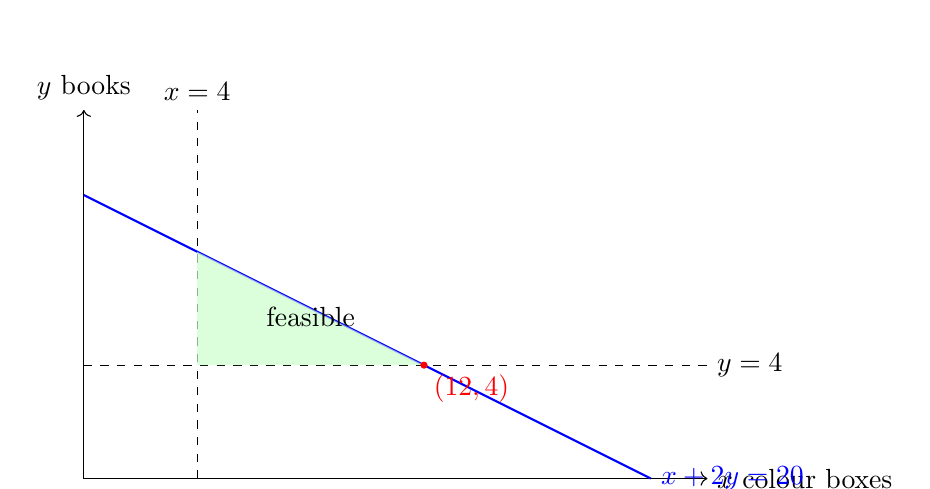
\begin{tikzpicture}[scale=0.36]
\draw[->] (0,0) -- (22,0) node[right] {$x$ colour boxes};
\draw[->] (0,0) -- (0,13) node[above] {$y$ books};
\draw[thick,blue] (0,10) -- (20,0) node[right] {$x+2y=20$};
\draw[dashed] (4,0) -- (4,13) node[above] {$x=4$};
\draw[dashed] (0,4) -- (22,4) node[right] {$y=4$};
\fill[green!20,opacity=0.7] (4,4) -- (12,4) -- (4,8) -- cycle;
\filldraw[red] (12,4) circle (3pt) node[below right] {$(12,4)$};
\node at (8,5.7) {feasible};
\end{tikzpicture}
\end{center}
\finalans{12\text{ colour boxes and }4\text{ books; maximum items }=16}
\eanswer

\section*{Question 2}
\addcontentsline{toc}{section}{Question 2}

\question{(a) Using elementary row operations, find inverse of
\[
A=\begin{bmatrix}1&2&2\\2&1&2\\2&2&1\end{bmatrix}.
\]}
\answer
We augment \(A\) with \(I_3\):
\[
\left[\begin{array}{ccc|ccc}
1&2&2&1&0&0\\
2&1&2&0&1&0\\
2&2&1&0&0&1
\end{array}\right].
\]
Applying elementary row operations and reducing the left side to identity gives
\[
\left[\begin{array}{ccc|ccc}
1&0&0&-\frac35&\frac25&\frac25\\
0&1&0&\frac25&-\frac35&\frac25\\
0&0&1&\frac25&\frac25&-\frac35
\end{array}\right].
\]
Therefore,
\[
A^{-1}=\begin{bmatrix}
-\frac35&\frac25&\frac25\\
\frac25&-\frac35&\frac25\\
\frac25&\frac25&-\frac35
\end{bmatrix}.
\]
Equivalently,
\finalans{A^{-1}=\frac15\begin{bmatrix}-3&2&2\\2&-3&2\\2&2&-3\end{bmatrix}}
\eanswer

\question{(b) If \(x=3+2i\), find the value of
\[
x^4-4x^3+4x^2+8x+40.
\]}
\answer
Substitute \(x=3+2i\). First,
\[
x^2=(3+2i)^2=9+12i+4i^2=5+12i.
\]
Then
\[
x^3=x^2x=(5+12i)(3+2i)=15+10i+36i+24i^2=-9+46i.
\]
Also
\[
x^4=x^3x=(-9+46i)(3+2i)=-27-18i+138i+92i^2=-119+120i.
\]
Now
\begin{align*}
x^4-4x^3+4x^2+8x+40
&=(-119+120i)-4(-9+46i)+4(5+12i)+8(3+2i)+40\\
&=(-119+120i)+(36-184i)+(20+48i)+(24+16i)+40\\
&=1+0i.
\end{align*}
\finalans{1}
\eanswer

\question{(c) Find the sum of an infinite G.P. whose first term is 15 and fourth term is \(\frac{3}{25}\).}
\answer
Let the first term be \(a=15\) and common ratio be \(r\). The fourth term is
\[
ar^3=\frac{3}{25}.
\]
Thus
\[
15r^3=\frac{3}{25}
\quad\Rightarrow\quad
r^3=\frac{3}{25\cdot15}=\frac{1}{125}.
\]
Hence
\[
r=\frac15.
\]
The sum of an infinite G.P. is
\[
S_\infty=\frac{a}{1-r},\qquad |r|<1.
\]
So
\[
S_\infty=\frac{15}{1-\frac15}=\frac{15}{\frac45}=\frac{75}{4}.
\]
\finalans{\frac{75}{4}}
\eanswer

\question{(d) If \(\alpha\) and \(\beta\) are roots of \(x^2-4x+5=0\), find the quadratic equation whose roots are \(\alpha^2+3\) and \(\beta^2+3\).}
\answer
For
\[
x^2-4x+5=0,
\]
we have
\[
\alpha+\beta=4,
\qquad \alpha\beta=5.
\]
New roots are
\[
\alpha^2+3,
\qquad \beta^2+3.
\]
Their sum is
\[
(\alpha^2+3)+(\beta^2+3)=\alpha^2+\beta^2+6.
\]
Now
\[
\alpha^2+\beta^2=(\alpha+\beta)^2-2\alpha\beta=16-10=6.
\]
So the sum of new roots is
\[
6+6=12.
\]
Their product is
\[
(\alpha^2+3)(\beta^2+3)=\alpha^2\beta^2+3(\alpha^2+\beta^2)+9.
\]
Therefore,
\[
=5^2+3(6)+9=25+18+9=52.
\]
Hence required equation is
\finalans{x^2-12x+52=0}
\eanswer

\section*{Question 3}
\addcontentsline{toc}{section}{Question 3}

\question{(a) Find
\[
\lim_{x\to 0}\frac{\sqrt{x+5}-\sqrt5}{\sqrt{x}}.
\]}
\answer
Rationalize the numerator:
\[
\frac{\sqrt{x+5}-\sqrt5}{\sqrt{x}}\cdot
\frac{\sqrt{x+5}+\sqrt5}{\sqrt{x+5}+\sqrt5}
=\frac{x}{\sqrt{x}(\sqrt{x+5}+\sqrt5)}.
\]
Thus
\[
\frac{\sqrt{x+5}-\sqrt5}{\sqrt{x}}
=\frac{\sqrt{x}}{\sqrt{x+5}+\sqrt5}.
\]
Taking \(x\to0^+\),
\[
\lim_{x\to0^+}\frac{\sqrt{x}}{\sqrt{x+5}+\sqrt5}=\frac{0}{2\sqrt5}=0.
\]
\finalans{0}
\eanswer

\question{(b) If
\[
y=\left[x(x-1)(x+2)\right]^{5/7},
\]
find \(\frac{dy}{dx}\).}
\answer
Let
\[
u=x(x-1)(x+2).
\]
Then
\[
y=u^{5/7}.
\]
Now
\[
u=x(x^2+x-2)=x^3+x^2-2x,
\]
so
\[
\frac{du}{dx}=3x^2+2x-2.
\]
By chain rule,
\[
\frac{dy}{dx}=\frac{5}{7}u^{-2/7}\frac{du}{dx}.
\]
Therefore,
\finalans{\frac{dy}{dx}=\frac{5(3x^2+2x-2)}{7\left[x(x-1)(x+2)\right]^{2/7}}}
\eanswer

\question{(c) Find the local extrema of
\[
f(x)=\frac34x^4-8x^3+\frac{45}{2}x^2+105.
\]}
\answer
Differentiate:
\[
f'(x)=3x^3-24x^2+45x=3x(x^2-8x+15).
\]
Therefore,
\[
f'(x)=3x(x-3)(x-5).
\]
Critical points are
\[
x=0,3,5.
\]
Second derivative is
\[
f''(x)=9x^2-48x+45.
\]
Now
\[
f''(0)=45>0,
\]
so \(x=0\) is a local minimum. Also
\[
f''(3)=81-144+45=-18<0,
\]
so \(x=3\) is a local maximum. Finally,
\[
f''(5)=225-240+45=30>0,
\]
so \(x=5\) is a local minimum.

Function values:
\[
f(0)=105,
\qquad f(3)=\frac{609}{4},
\qquad f(5)=\frac{545}{4}.
\]
\finalans{\text{Local minima: }(0,105),(5,545/4);\quad \text{local maximum: }(3,609/4)}
\begin{center}
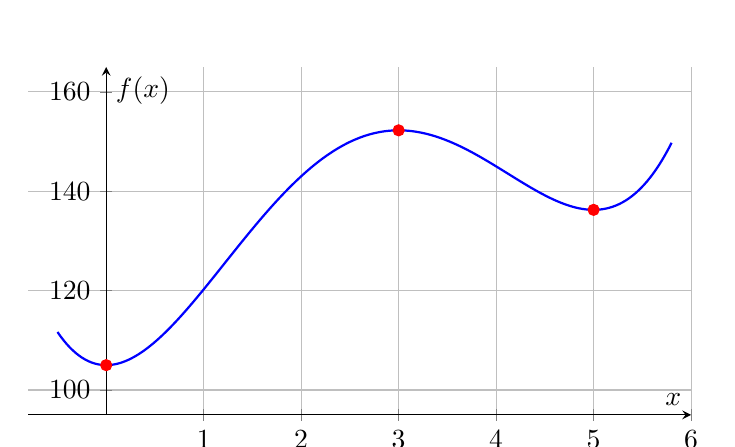
\begin{tikzpicture}
\begin{axis}[width=10cm,height=6cm,axis lines=middle,xmin=-0.8,xmax=6,ymin=95,ymax=165,grid=both,xlabel={$x$},ylabel={$f(x)$},samples=200]
\addplot[blue,thick,domain=-0.5:5.8]{0.75*x^4-8*x^3+22.5*x^2+105};
\addplot[only marks,red] coordinates {(0,105) (3,152.25) (5,136.25)};
\end{axis}
\end{tikzpicture}
\end{center}
\eanswer

\question{(d) If
\[
y=ax+\frac{b}{x},
\]
show that
\[
x^2\frac{d^2y}{dx^2}+x\frac{dy}{dx}-y=0.
\]}
\answer
Given
\[
y=ax+bx^{-1}.
\]
Differentiate:
\[
\frac{dy}{dx}=a-bx^{-2}=a-\frac{b}{x^2}.
\]
Again,
\[
\frac{d^2y}{dx^2}=2bx^{-3}=\frac{2b}{x^3}.
\]
Now
\begin{align*}
x^2\frac{d^2y}{dx^2}+x\frac{dy}{dx}-y
&=x^2\left(\frac{2b}{x^3}\right)+x\left(a-\frac{b}{x^2}\right)-\left(ax+\frac{b}{x}\right)\\
&=\frac{2b}{x}+ax-\frac{b}{x}-ax-\frac{b}{x}\\
&=0.
\end{align*}
Hence proved.
\eanswer

\section*{Question 4}
\addcontentsline{toc}{section}{Question 4}

\question{(a) Evaluate
\[
\int x\sqrt{x+2}\,dx.
\]}
\answer
Put
\[
u=x+2\quad\Rightarrow\quad x=u-2,\quad dx=du.
\]
Then
\[
\int x\sqrt{x+2}\,dx=\int (u-2)u^{1/2}\,du.
\]
So
\[
=\int \left(u^{3/2}-2u^{1/2}\right)du
=\frac{2}{5}u^{5/2}-\frac{4}{3}u^{3/2}+C.
\]
Substituting \(u=x+2\),
\finalans{\int x\sqrt{x+2}\,dx=\frac{2}{5}(x+2)^{5/2}-\frac{4}{3}(x+2)^{3/2}+C}
\eanswer

\question{(b) Evaluate
\[
\int_0^1\frac{x}{\sqrt{1-x^2}}\,dx.
\]}
\answer
Let
\[
u=1-x^2\quad\Rightarrow\quad du=-2x\,dx.
\]
Therefore,
\[
x\,dx=-\frac12du.
\]
When \(x=0\), \(u=1\). When \(x=1\), \(u=0\). Hence
\[
\int_0^1\frac{x}{\sqrt{1-x^2}}\,dx
=-\frac12\int_1^0u^{-1/2}\,du
=\frac12\int_0^1u^{-1/2}\,du.
\]
Thus
\[
=\frac12\left[2u^{1/2}\right]_0^1=1.
\]
\finalans{1}
\eanswer

\question{(c) Find the length of the curve \(y=4+3x\), from \((0,4)\) to \((2,10)\).}
\answer
For a curve \(y=f(x)\), arc length from \(x=a\) to \(x=b\) is
\[
L=\int_a^b\sqrt{1+\left(\frac{dy}{dx}\right)^2}\,dx.
\]
Here
\[
y=4+3x\quad\Rightarrow\quad \frac{dy}{dx}=3.
\]
From \((0,4)\) to \((2,10)\), \(x\) runs from 0 to 2. Hence
\[
L=\int_0^2\sqrt{1+3^2}\,dx=\int_0^2\sqrt{10}\,dx=2\sqrt{10}.
\]
\finalans{2\sqrt{10}}
\begin{center}
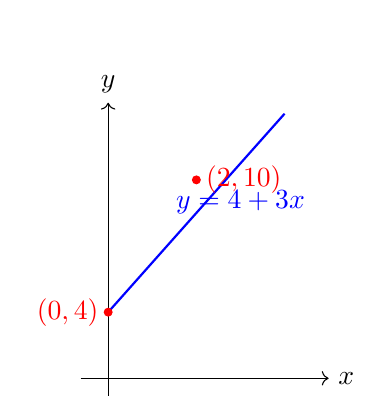
\begin{tikzpicture}[scale=0.7]
\draw[->] (-0.5,0) -- (4,0) node[right] {$x$};
\draw[->] (0,-0.5) -- (0,5) node[above] {$y$};
\draw[thick,blue] (0,1.2) -- (3.2,4.8);
\filldraw[red] (0,1.2) circle (2pt) node[left] {$(0,4)$};
\filldraw[red] (1.6,3.6) circle (2pt) node[right] {$(2,10)$};
\node[blue] at (2.4,3.2) {$y=4+3x$};
\end{tikzpicture}
\end{center}
\eanswer

\question{(d) Show that
\[
(\vec a\times\vec b)\cdot(\vec c\times\vec d)=(\vec a\cdot\vec c)(\vec b\cdot\vec d)-(\vec a\cdot\vec d)(\vec b\cdot\vec c).
\]}
\answer
This is the vector product scalar product identity. Using the determinant form of scalar triple products,
\[
(\vec a\times\vec b)\cdot(\vec c\times\vec d)
=\begin{vmatrix}
\vec a\cdot\vec c & \vec a\cdot\vec d\\
\vec b\cdot\vec c & \vec b\cdot\vec d
\end{vmatrix}.
\]
Expanding the determinant,
\[
(\vec a\times\vec b)\cdot(\vec c\times\vec d)
=(\vec a\cdot\vec c)(\vec b\cdot\vec d)-(\vec a\cdot\vec d)(\vec b\cdot\vec c).
\]
Hence proved.
\eanswer

\section*{Question 5}
\addcontentsline{toc}{section}{Question 5}

\question{(a) Find the shortest distance between the lines
\[
\frac{x-1}{2}=\frac{y+1}{3}=z
\]
and
\[
\frac{x+1}{5}=\frac{y-2}{1}=\frac{z-2}{0}.
\]}
\answer
For the first line,
\[
\frac{x-1}{2}=\frac{y+1}{3}=z=t,
\]
so a point and direction vector are
\[
P_1=(1,-1,0),\qquad \vec d_1=(2,3,1).
\]
For the second line,
\[
\frac{x+1}{5}=\frac{y-2}{1}=\frac{z-2}{0}=s,
\]
so
\[
P_2=(-1,2,2),\qquad \vec d_2=(5,1,0).
\]
The shortest distance between two skew lines is
\[
D=\frac{|(P_2-P_1)\cdot(\vec d_1\times\vec d_2)|}{|\vec d_1\times\vec d_2|}.
\]
Now
\[
P_2-P_1=(-2,3,2),
\]
and
\[
\vec d_1\times\vec d_2=
\begin{vmatrix}
\hat i&\hat j&\hat k\\
2&3&1\\
5&1&0
\end{vmatrix}=(-1,5,-13).
\]
Thus
\[
(P_2-P_1)\cdot(\vec d_1\times\vec d_2)=(-2,3,2)\cdot(-1,5,-13)=2+15-26=-9.
\]
So absolute value is 9. Also
\[
|\vec d_1\times\vec d_2|=\sqrt{(-1)^2+5^2+(-13)^2}=\sqrt{195}.
\]
Therefore,
\finalans{D=\frac{9}{\sqrt{195}}}
\eanswer

\question{(b) Solve the inequality
\[
\left|\frac{2x-1}{3}\right|\le2.
\]}
\answer
Using \(|A|\le k\Rightarrow -k\le A\le k\), we get
\[
-2\le \frac{2x-1}{3}\le 2.
\]
Multiplying by 3,
\[
-6\le 2x-1\le 6.
\]
Adding 1,
\[
-5\le 2x\le 7.
\]
Dividing by 2,
\[
-\frac52\le x\le \frac72.
\]
\finalans{x\in\left[-\frac52,\frac72\right]}
\begin{center}
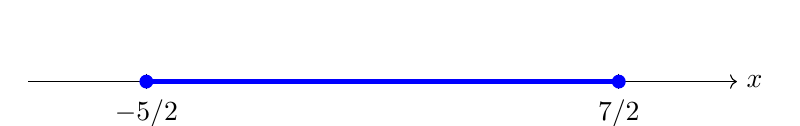
\begin{tikzpicture}
\draw[->] (-4,0) -- (5,0) node[right] {$x$};
\draw (-2.5,0.1)--(-2.5,-0.1) node[below] {$-5/2$};
\draw (3.5,0.1)--(3.5,-0.1) node[below] {$7/2$};
\draw[line width=2pt,blue] (-2.5,0) -- (3.5,0);
\fill[blue] (-2.5,0) circle (2.5pt);
\fill[blue] (3.5,0) circle (2.5pt);
\end{tikzpicture}
\end{center}
\eanswer

\question{(c) Using determinants, show that the points
\[
A(a,b+c),\quad B(b,c+a),\quad C(c,a+b)
\]
are collinear.}
\answer
Three points \((x_1,y_1),(x_2,y_2),(x_3,y_3)\) are collinear if
\[
\begin{vmatrix}
x_1&y_1&1\\
x_2&y_2&1\\
x_3&y_3&1
\end{vmatrix}=0.
\]
Here
\[
\Delta=
\begin{vmatrix}
a&b+c&1\\
b&c+a&1\\
c&a+b&1
\end{vmatrix}.
\]
Apply the column operation
\[
C_2\to C_2+C_1.
\]
Then
\[
C_2=\begin{bmatrix}a+b+c\\a+b+c\\a+b+c\end{bmatrix}.
\]
Thus
\[
\Delta=(a+b+c)
\begin{vmatrix}
a&1&1\\
b&1&1\\
c&1&1
\end{vmatrix}.
\]
The second and third columns are identical, so the determinant is zero. Therefore,
\[
\Delta=0.
\]
Hence the points are collinear.
\eanswer

\question{(d) If
\[
y=2e^x+e^{-x}
\]
and
\[
\frac{d^2y}{dx^2}=ky,
\]
find \(k\).}
\answer
Given
\[
y=2e^x+e^{-x}.
\]
Differentiate:
\[
\frac{dy}{dx}=2e^x-e^{-x}.
\]
Differentiate again:
\[
\frac{d^2y}{dx^2}=2e^x+e^{-x}.
\]
But
\[
y=2e^x+e^{-x}.
\]
Therefore,
\[
\frac{d^2y}{dx^2}=y.
\]
Comparing with
\[
\frac{d^2y}{dx^2}=ky,
\]
we get
\finalans{k=1}
\eanswer

\newpage
\section*{Theory and Formula Sheet}
\addcontentsline{toc}{section}{Theory and Formula Sheet}

\begin{tcolorbox}[breakable,colback=lightgray,colframe=titleblue,title=Key Theory Required for This Paper]
\textbf{1. Determinants}
\begin{itemize}[leftmargin=1.2em]
\item If two rows or two columns of a determinant are identical, its value is zero.
\item If a row/column operation of the type \(R_i\to R_i+kR_j\) or \(C_i\to C_i+kC_j\) is applied, the determinant does not change.
\item Three points \((x_1,y_1),(x_2,y_2),(x_3,y_3)\) are collinear if
\[
\begin{vmatrix}x_1&y_1&1\\x_2&y_2&1\\x_3&y_3&1\end{vmatrix}=0.
\]
\end{itemize}

\textbf{2. Matrices}
\begin{itemize}[leftmargin=1.2em]
\item For a polynomial \(f(x)=x^2-5x+6\), \(f(A)=A^2-5A+6I\).
\item To find \(A^{-1}\) by elementary row operations, reduce \([A\mid I]\) to \([I\mid A^{-1}]\).
\end{itemize}

\textbf{3. Mathematical Induction}
\begin{itemize}[leftmargin=1.2em]
\item Step 1: Prove the result for \(n=1\).
\item Step 2: Assume true for \(n=k\).
\item Step 3: Prove true for \(n=k+1\).
\end{itemize}

\textbf{4. Sequences and Series}
\begin{itemize}[leftmargin=1.2em]
\item Geometric progression: \(a,ar,ar^2,\ldots\).
\item Sum of infinite G.P.: \(S_\infty=\frac{a}{1-r}\), where \(|r|<1\).
\item \(9,99,999,\ldots\) has \(r\)-th term \(10^r-1\).
\end{itemize}

\textbf{5. Quadratic Equations}
\begin{itemize}[leftmargin=1.2em]
\item If roots are \(\alpha,\beta\), then
\[
\alpha+\beta=-\frac{b}{a},\qquad \alpha\beta=\frac{c}{a}.
\]
\item Equation with roots \(p,q\) is
\[
x^2-(p+q)x+pq=0.
\]
\end{itemize}

\textbf{6. Complex Numbers}
\begin{itemize}[leftmargin=1.2em]
\item If \(z=x+iy\), then \(\operatorname{Re}(z)=x\) and \(\operatorname{Im}(z)=y\).
\item \(|x+iy|=\sqrt{x^2+y^2}\).
\end{itemize}

\textbf{7. Differentiation}
\begin{itemize}[leftmargin=1.2em]
\item Chain rule: if \(y=[u(x)]^n\), then \(\frac{dy}{dx}=n[u(x)]^{n-1}u'(x)\).
\item Local extrema occur where \(f'(x)=0\). If \(f''(x)>0\), local minimum; if \(f''(x)<0\), local maximum.
\end{itemize}

\textbf{8. Integration and Arc Length}
\begin{itemize}[leftmargin=1.2em]
\item Substitution method is useful when an expression and its derivative occur together.
\item Arc length of \(y=f(x)\) from \(x=a\) to \(x=b\):
\[
L=\int_a^b\sqrt{1+\left(\frac{dy}{dx}\right)^2}\,dx.
\]
\end{itemize}

\textbf{9. Vectors and 3-D Geometry}
\begin{itemize}[leftmargin=1.2em]
\item Shortest distance between skew lines:
\[
D=\frac{|(P_2-P_1)\cdot(\vec d_1\times\vec d_2)|}{|\vec d_1\times\vec d_2|}.
\]
\item Vector identity:
\[
(\vec a\times\vec b)\cdot(\vec c\times\vec d)=(\vec a\cdot\vec c)(\vec b\cdot\vec d)-(\vec a\cdot\vec d)(\vec b\cdot\vec c).
\]
\item In a rhombus with adjacent side vectors \(\vec a,\vec b\), diagonals are \(\vec a+\vec b\) and \(\vec a-\vec b\); their dot product is \(|\vec a|^2-|\vec b|^2=0\).
\end{itemize}

\textbf{10. Linear Programming}
\begin{itemize}[leftmargin=1.2em]
\item Convert word problem into inequalities.
\item The maximum or minimum of a linear objective function occurs at a corner point of the feasible region.
\end{itemize}
\end{tcolorbox}

\end{document}
